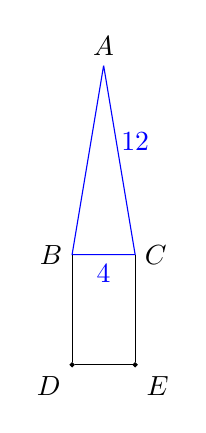
\begin{tikzpicture}
[scale=.2,>=stealth,point/.style={draw,circle,fill = black,inner sep=0.5pt},]

%Triangle sides
\def\a{4}
\def\b{7}
\def\c{3}
\def\d{2}
\def\e{19}

%Marking coordiantes
\color{black}
\coordinate [label=above:$A$] (A) at (\d,\e);
\coordinate [label=left:$B$] (B) at (0,\b);
\coordinate [label=right:$C$] (C) at (\a,\b);



%Drawing triangle ABC
\color{blue}
\draw (A) -- node[left] {$\textrm{}$} (B) -- node[below] {$\textrm{4}$} (C) -- node[above,,xshift=2mm] {$\textrm{12}$} (A);
\color{black}
\node (D) at (0, 0)[point,label=below left:$D$] {} ;
\node (E) at (\a, 0)[point,label=below right:$E$] {};

%Joining BD, CE and DE
\draw (B)--(D) ;
\draw (C)--(E);
\draw (D)--(E);

\end{tikzpicture}